%!TEX root=../index.tex

\chapter{Rilevamento}
\label{chap:rilevamento}
    I classificatori, ottenuti in fase di allenamento e parametrizzati in fase di validazione, non sono direttamente utilizzabili per il rilevamento delle persone all'interno di un frame di profondità.
    Basti pensare al fatto che ogni classificatore viene allenato con immagini di $24 \times 24$ pixel, di conseguenza, tutti i meccanismi sviluppati dall'algoritmo di apprendimento per il rilevamento, sono indissolubilmente legati a tale dimensione.

    Nel capitolo \ref{chap:features}, introducendo le feature di Haar, è stato necessario modificarne la formula di calcolo al fine di minimizzare la sensibilità rispetto ai ridimensionamenti della feature stessa.
    Il motivo per cui è necessario ridimensionare una feature è esattamente questo: i classificatori vengono allenati con immagini di profondità molto piccole, ma vengono trasformati in blocco per riuscire ad elaborare immagini di dimensione maggiore.

    Dopo tale trasformazione, i classificatori riusciranno comunque ad elaborare delle porzioni di immagini di profondità che al massimo potranno contenere una persona: bisognerà tener conto anche di tale aspetto.

    \section{Tecnica di Rilevamento}
    \label{sec:detection_tecnique}
        Vengono create delle \emph{detection window} per gestire il rilevamento su frame.
        La detection window non è altro che una finestra, una porzione dell'immagine di profondità che viene data in pasto ai classificatori per determinare se essa contiene o meno l'immagine di una persona.

        Per fare ciò è necessario, innanzi tutto, ridimensionare correttamente l'intero classificatore in modo tale da rendere la dimensione delle immagini in input compatibili con la dimensione delle figure HASP nel frame di profondità.

        È stato accennato in precedenza che l'immagine HASP della persona, in un frame ripreso con il Kinect V2, viene circoscritta da un'area quadrata di dimensione variabile tra i $120 \times 120$ e i $160 \times 160$ pixel, dipendentemente dalla statura e dalla corporatura del soggetto.

        Viene presentato, di seguito, l'algoritmo per il ridimensionamento dei classificatori forti. 
        Si tenga presente che, al livello di strutture dati, uno strong learner non è altro che una collezione di weak learner correlata dei relativi fattori moltiplicativi e da un valore di soglia.
        A loro volta, i weak learner non sono altro che delle feature di haar (tipo della feature, cordinate dell'area rettangolare che racchiude interamente la feature), correlate da un valore di soglia e di una polarità.
        Alla luce di tali considerazioni, ridimensionare un classificatore non vuol dire altro che ridimensionare le feature relative ai weak learner a lui associati.

        \begin{enumerate}
            \item \emph{For each} weak learner $w_i \in \Phi = \left\{w_1, \cdots, w_k\right\}$: 
            \begin{enumerate}
                \item Sia $f$ la feature associata al weak learner $w_i$.
                Quest'ultima è racchiusa in una regione rettangolare $R$, esprimibile, rispetto al sistema di coordinate convenzionale delle immagini raster, in base alle coordinate del punto in alto a sinistra (\emph{Top Left Point}) e alle dimensioni del rettagolo (\emph{width} e \emph{height}).
                \begin{equation}
                    \label{subeq:rectangular_region}
                    R := (TLP, DIM) \text{ con } TLP = (tl_x, tl_y) \text{ e } DIM = (w, h)
                \end{equation}

                \item Siano ${W}^{'}_{w}$ e ${W}^{'}_{h}$ le nuove dimensioni desiderate per la finestra di classificazione.
                Essendo la finestra quadrata, si ha ${W}^{'}_{w} = {W}^{'}_{h} = W^{'}$.

                \item Si calcola il rapporto di ridimensionamento (si tenga a mente che il lato della finestra di classificazione originale è di $24$ pixel):
                \begin{equation}
                    \label{subeq:scale_ratio}
                    \sigma = \frac{W^{'}}{W} = \frac{W^{'}}{24}
                \end{equation}

                \item Si modifica la feature $f$ cambiando la posizione e la dimensione della regione rettangolare associata in modo da mantenere la proporzione con le nuove dimensioni desiderate\footnote{La notazione $\lfloor x \rfloor$ denota la parte intera di $x$.}:
                \begin{equation}
                    \label{subeq:resize}
                    R^{'} :=
                    \begin{cases}
                        tl^{'}_x = \lfloor \sigma tl_x \rfloor \\ 
                        tl^{'}_y = \lfloor \sigma tl_y \rfloor \\
                        w^{'} = \lfloor \sigma w \rfloor \\
                        h^{'} = \lfloor \sigma h \rfloor \\
                    \end{cases}
                \end{equation}

                \item Ad ogni feature è associato un tipo che ne identifica la forma.
                Si è parlato dei diversi tipi di feature nella sottosezione \ref{sub:haar_features_applications}: ad ognuno di essi è associato un vincolo di divisibilità rispetto una delle due dimensioni.
                Bisogna correggere le dimensioni della regione $R'$ affinchè questo vincolo venga soddisfatto (si fa riferimento alla figura \ref{fig:opencv_haar_features}.
                \begin{enumerate}
                    \item se $f$ è del tipo \ref{fig:opencv_haar_features}[1.a], allora:
                    \begin{equation}
                        w^{'} \leftarrow (w^{'} - \mod(w^{'}, 2))
                    \end{equation}

                    \item se $f$ è del tipo \ref{fig:opencv_haar_features}[1.b], allora:
                    \begin{equation}
                        h^{'} \leftarrow (h^{'} - \mod(h^{'}, 2))
                    \end{equation}

                    \item se $f$ è del tipo \ref{fig:opencv_haar_features}[2.a], allora:
                    \begin{equation}
                        w^{'} \leftarrow (w^{'} - \mod(w^{'}, 3))
                    \end{equation}

                    \item se $f$ è del tipo \ref{fig:opencv_haar_features}[2.c], allora:
                    \begin{equation}
                        h^{'} \leftarrow (h^{'} - \mod(h^{'}, 3))
                    \end{equation}
                \end{enumerate}
             \end{enumerate} 
        \end{enumerate}

        La possibilità di ridimensionare i classificatori risulta essere un vantaggio per quanto riguarda la scalabilità dell'applicazione.
        Attualmente una finestra di classificazione ha una dimensione statica, determinata empiricamente per riuscire a rilevare adeguatamente persone di corporatura e statura differenti.
        Tuttavia il sistema può essere migliorato andando a far variare la dimensione della finestra per garantire rilevamenti migliori.

        Una volta ottenuto un classificatore adattabile alla dimensione desiderata per la finestra di classificazione, è sufficiente far scorrere tale finestra in tutto il frame comprendone tutta l'aria, elaborando sequenzialmente tutto il frame.
        Ciò permette di effettuare delle rilevazioni in contesti statici, ovvero su singoli frame o su frame non correlati tra di loro.

        Quando si ha a che fare con frame correlati tra di loro, è possibile velocizzare il processo di rilevamento scartando delle intere aree del frame.

        Quando valgolo le precedenti ipotesi, infatti, dopo un'iniziale scansione totale del frame, l'algoritmo di rilevamento prende coscenza dell'eventuale presenza di persone e conosce a priori quali sono le zone in cui sicuramente, negli istanti successivi, tutte le finestre di rilevamento daranno esito negativo.

        Negli istanti successivi, vengono scansionate solamente le porzioni che si trovano nelle vicinanze della persona rilevata all'istante precedente.
        Si scansionano inoltre i bordi del frame, alla ricerca di eventuali persone in ingresso.
        Utilizzando questi accorgimenti, i tempi necessari al rilevamento su frame si accorciano notevolmente.

        % subsection sliding_della_detection_window (end)

    \section{Selezione della Finestra Migliore}
    \label{sec:best_detection_window}
        Solitamente, scansionando un frame alla ricerca di una persona, in prossimità di quest'ultima, saranno numerose le finestre di rilevamento che daranno esito positivo.
        Bisogna, di contro, elaborare un meccanismo di selezione della finestra migliore, che circoscriva adeguatamente l'area entro cui la persona si trova realmente.

        \begin{figure}[h]
            \centering
            \begin{subfigure}[b]{0.48\textwidth}
                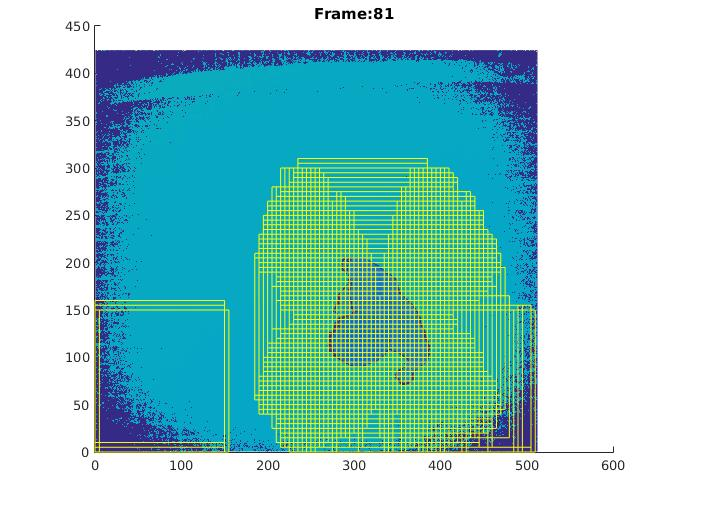
\includegraphics[width=\textwidth]{img/detection_without_selection.jpg}
                \caption{}
                \label{fig:detection_without_selection}
            \end{subfigure}
            ~ %add desired spacing between images, e. g. ~, \quad, \qquad, \hfill etc. 
              %(or a blank line to force the subfigure onto a new line)
            \begin{subfigure}[b]{0.48\textwidth}
                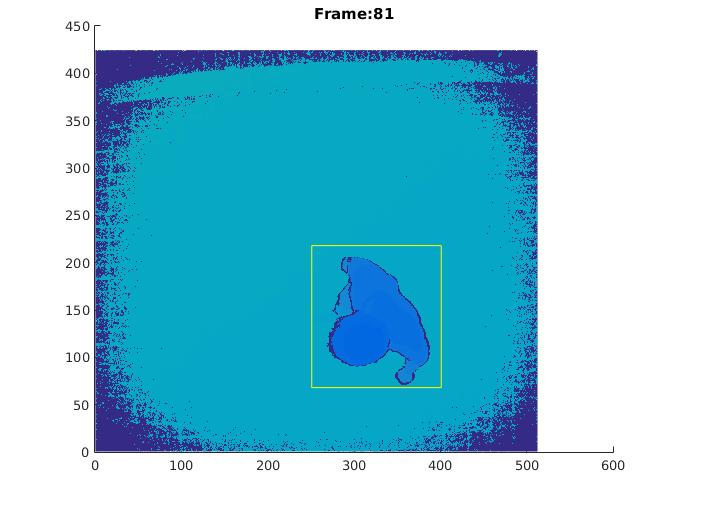
\includegraphics[width=\textwidth]{img/detection_with_selection.jpg}
                \caption{}
                \label{fig:detection_with_selection}
            \end{subfigure}
            \caption{Rilevamento senza selezione della finestra migliore \ref{fig:detection_without_selection} e con selezione \ref{fig:detection_with_selection}}
            \label{fig:detection}
        \end{figure}

        Il problema non è banale, allo stato attuale del sistema rappresenta a tutti gli effetti un collo di bottiglia per quanto riguarda la scalabilità.
        
        In prima approssimazione è stato utilizzato un algoritmo rudimentale basato sull'individuare il centro di una serie di finestre positive.
        Il risultato, seppur grezzo, è accettabile, grazie al bassissimo numero di falsi positivi prodotti dai classificatori. 

        In un secondo momento le finestre sono state pesate con valori decrescenti man mano che queste si allontanano dalla posizione della persona allo stato precedente.
        Finestre positive troppo distanti, difficilmente portano a risultati veritieri, quindi vengono premiate le finestre di rilevamento nelle immediate vicinanze della persona.
        Vengono inoltre effettuata una prima scrematura, non considerando rilevamenti che hanno prodotto un numero di finestre positive troppo basso.

        Lo svantaggio delle soluzioni appena presentate sta nel fatto che funzionano quando nel frame è presente una sola persona.
        Sarà necessario in futuro, per apportare dei miglioramenti, implementare una soluzione simile a quella descritta da Wang in \cite{Wang14}, basata sul raggruppamento delle finestre in insiemi di aree connesse tra loro e sulla selezione di quelle con un maggiore indice di sovrapposizione. 